% --------------------------------------
% labels: \label{mil2:res:[type]:[name]}
% --------------------------------------
% PAST TENSE

The free electron fraction as computed from the Saha and Peebles equations in their respective regimes is plotted in \cref{mil2:res:fig:electron_fraction}.
\begin{figure}[!ht]
    \centering
    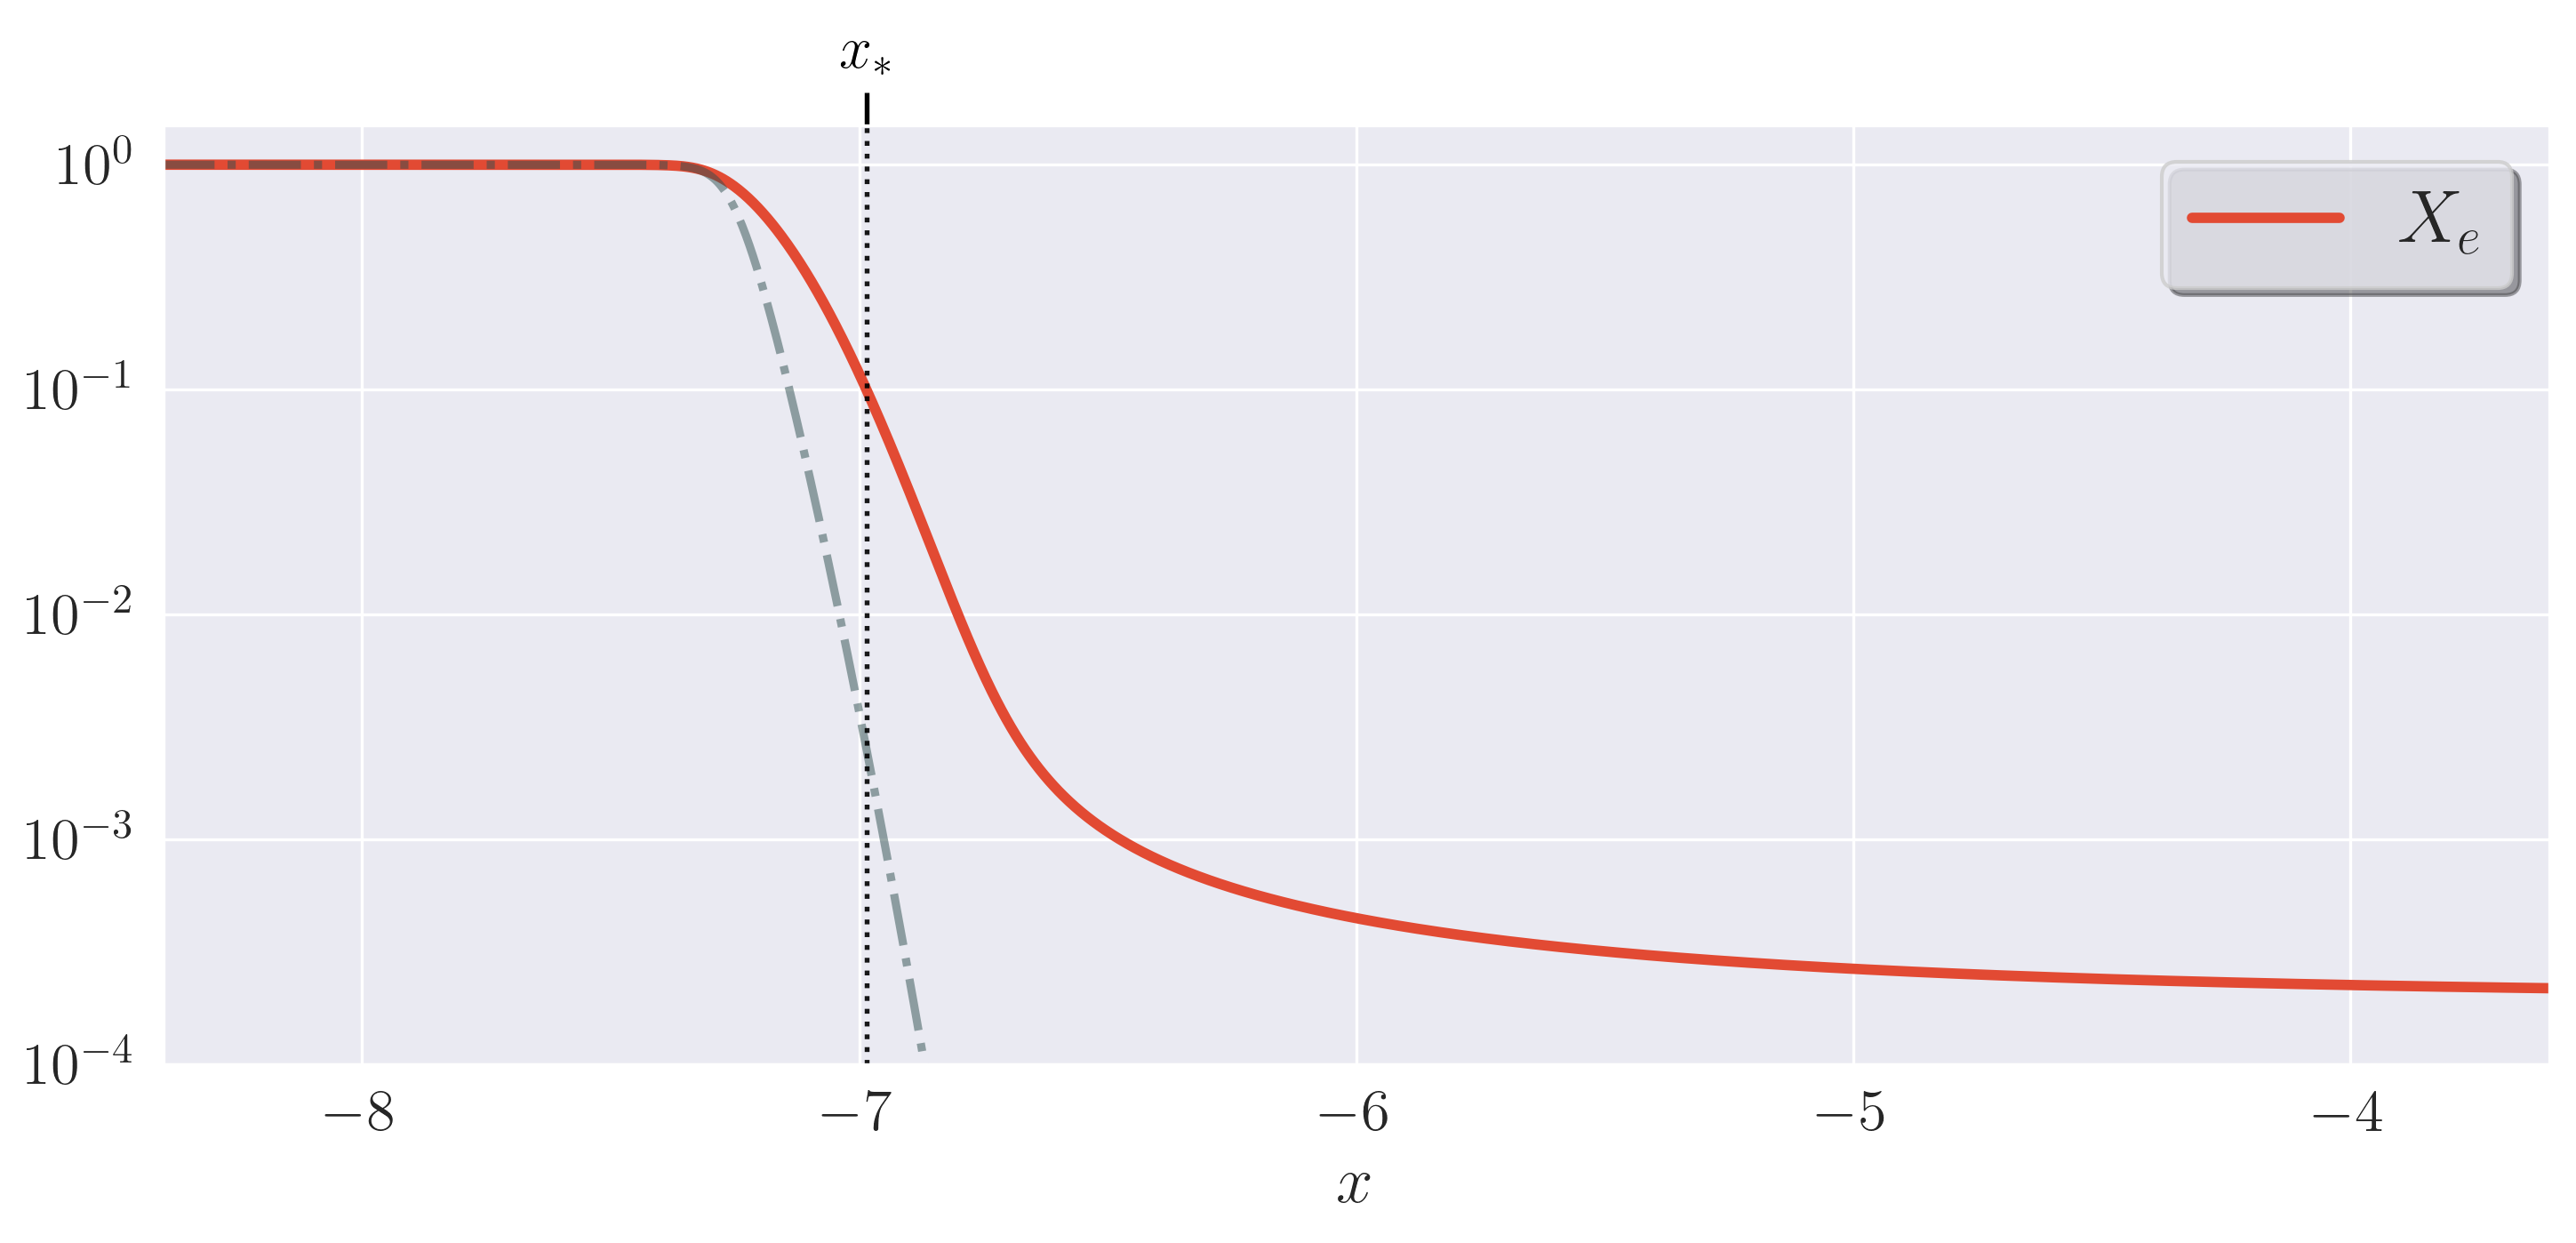
\includegraphics[width=\linewidth]{milestone2/electron_fraction.png} 
    \caption{\textcolor{blue}{The fractional electron density $X_e(x)$ resulting from the Peebles and Saha equations.}} 
    \label[fig]{mil2:res:fig:electron_fraction}
\end{figure}
As elaborated in \cref{mil2:imp:sec:tau_gt} we calculated the optical depth and visibility function and their derivatives.
We present the optical depth and its derivatives in \cref{mil2:res:fig:optical_depth}. The visibility function is demonstrated in \cref{mil2:res:fig:visibility_function} scaled to be comparable to its (also scaled) derivatives.
\begin{figure}[!ht]
    \centering
    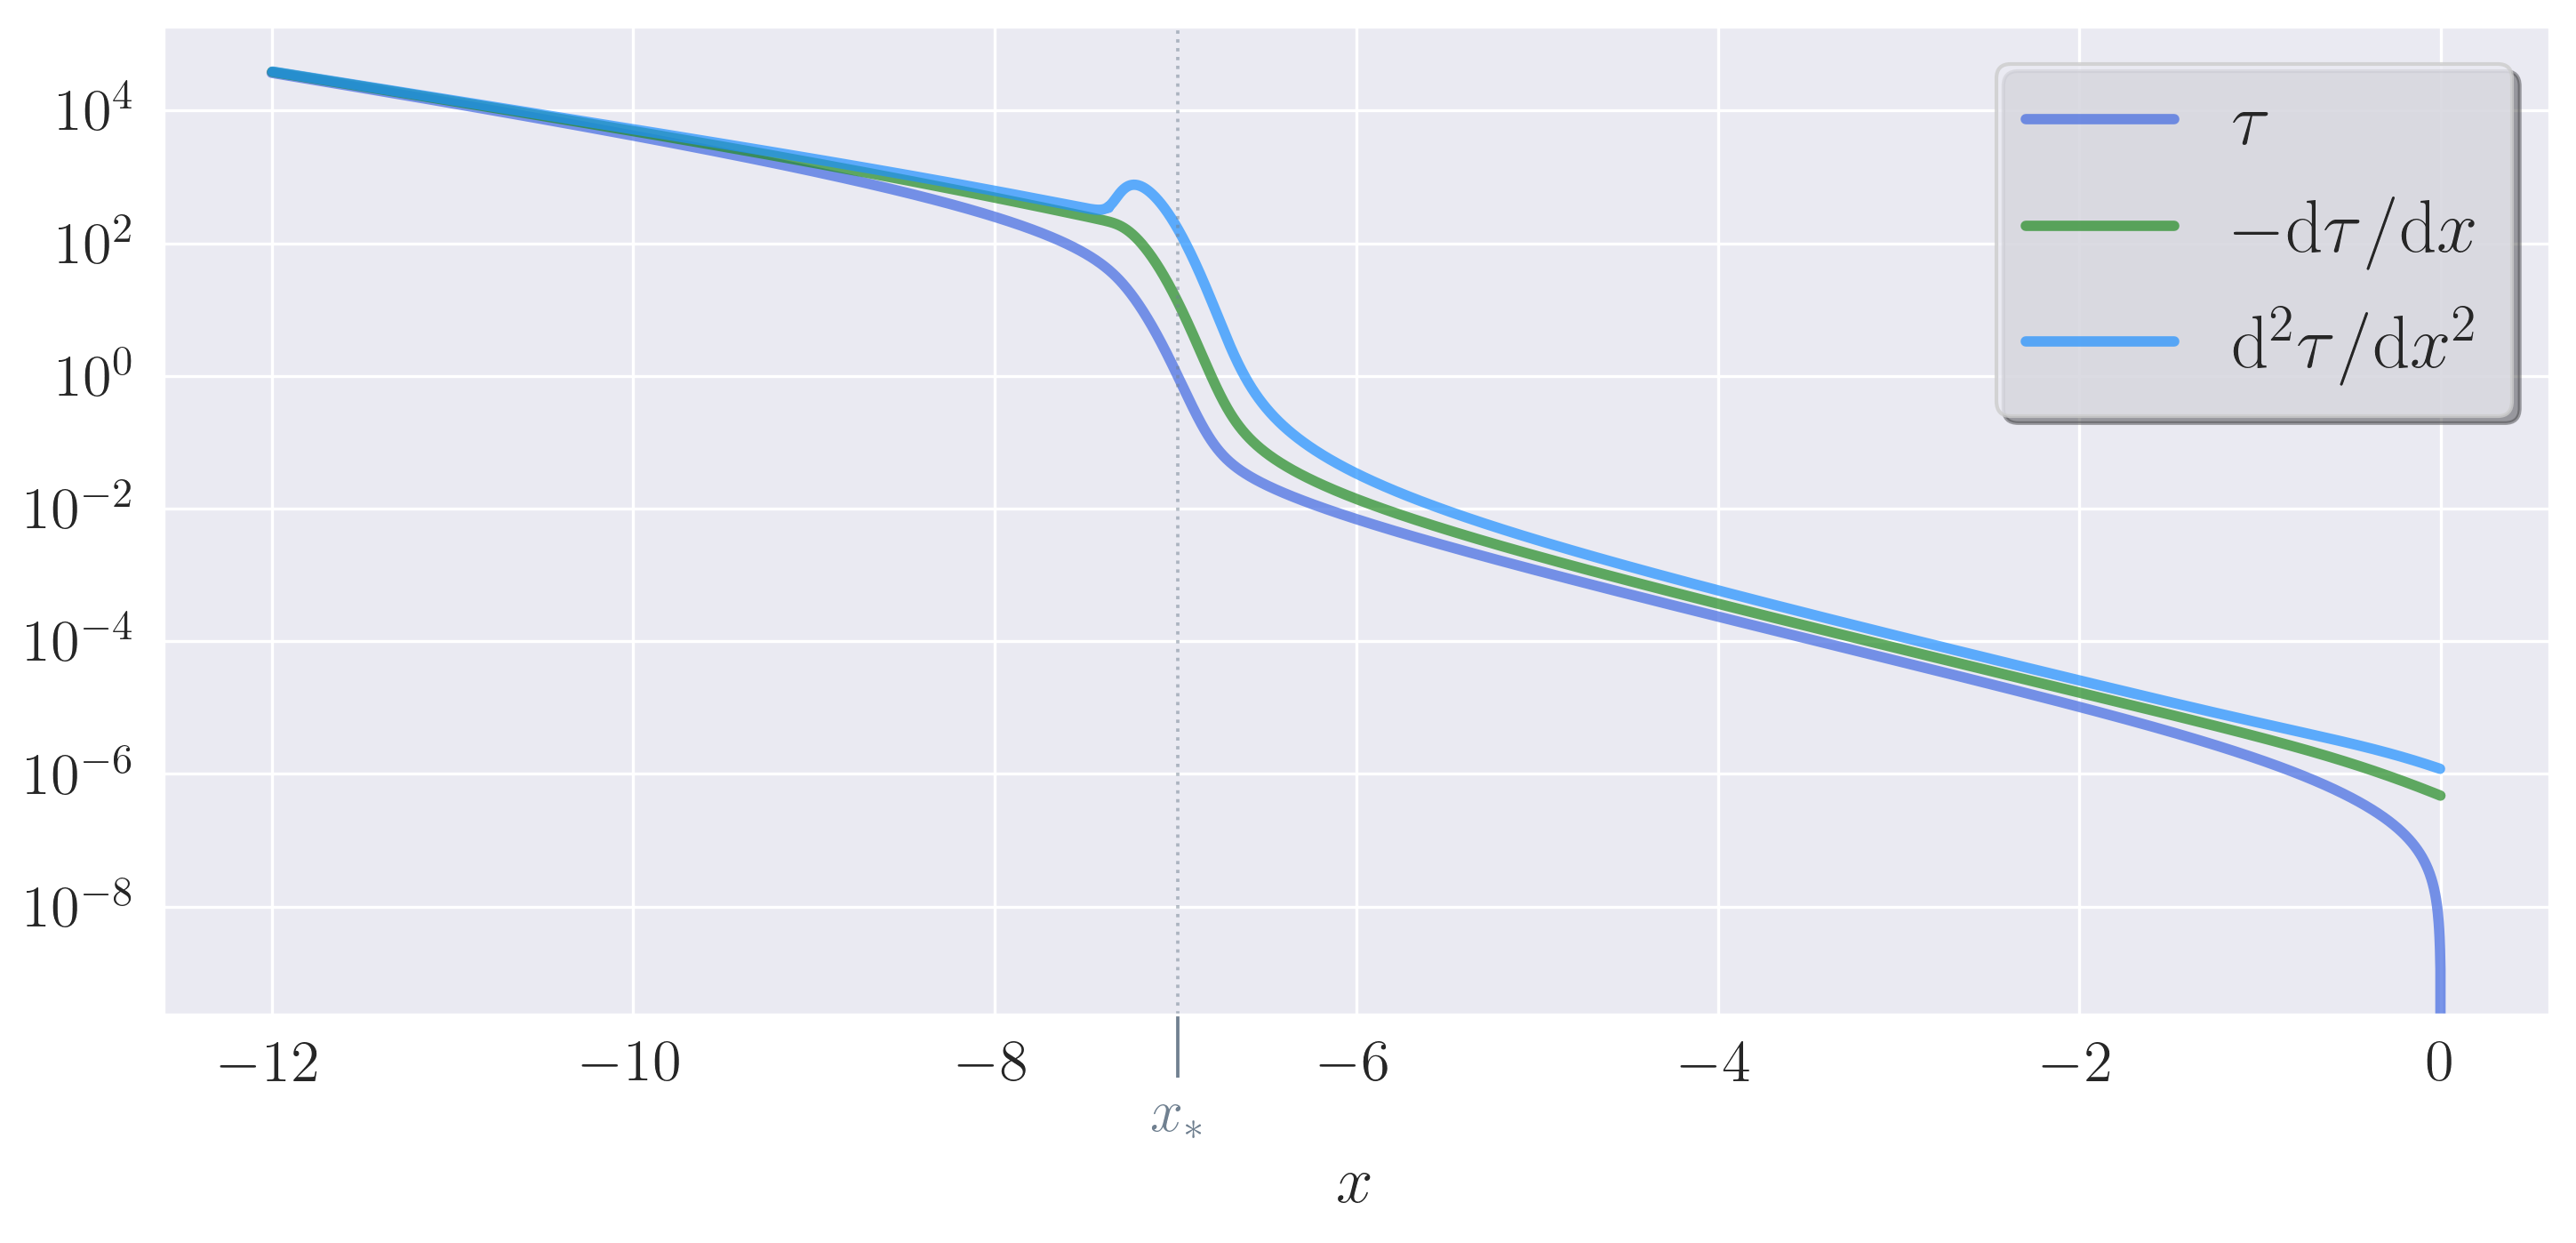
\includegraphics[width=\linewidth]{milestone2/optical_depth_misc.png} 
    \caption{\textcolor{blue}{The optical depth $\tau(x)$ and its derivatives $-\dv{\tau(x)}{x}$ and $\dv[2]{\tau(x)}{x}$ as functions of logarithmic scale factor $x$.}} 
    \label[fig]{mil2:res:fig:optical_depth}
\end{figure}
\begin{figure}[!ht]
    \centering
    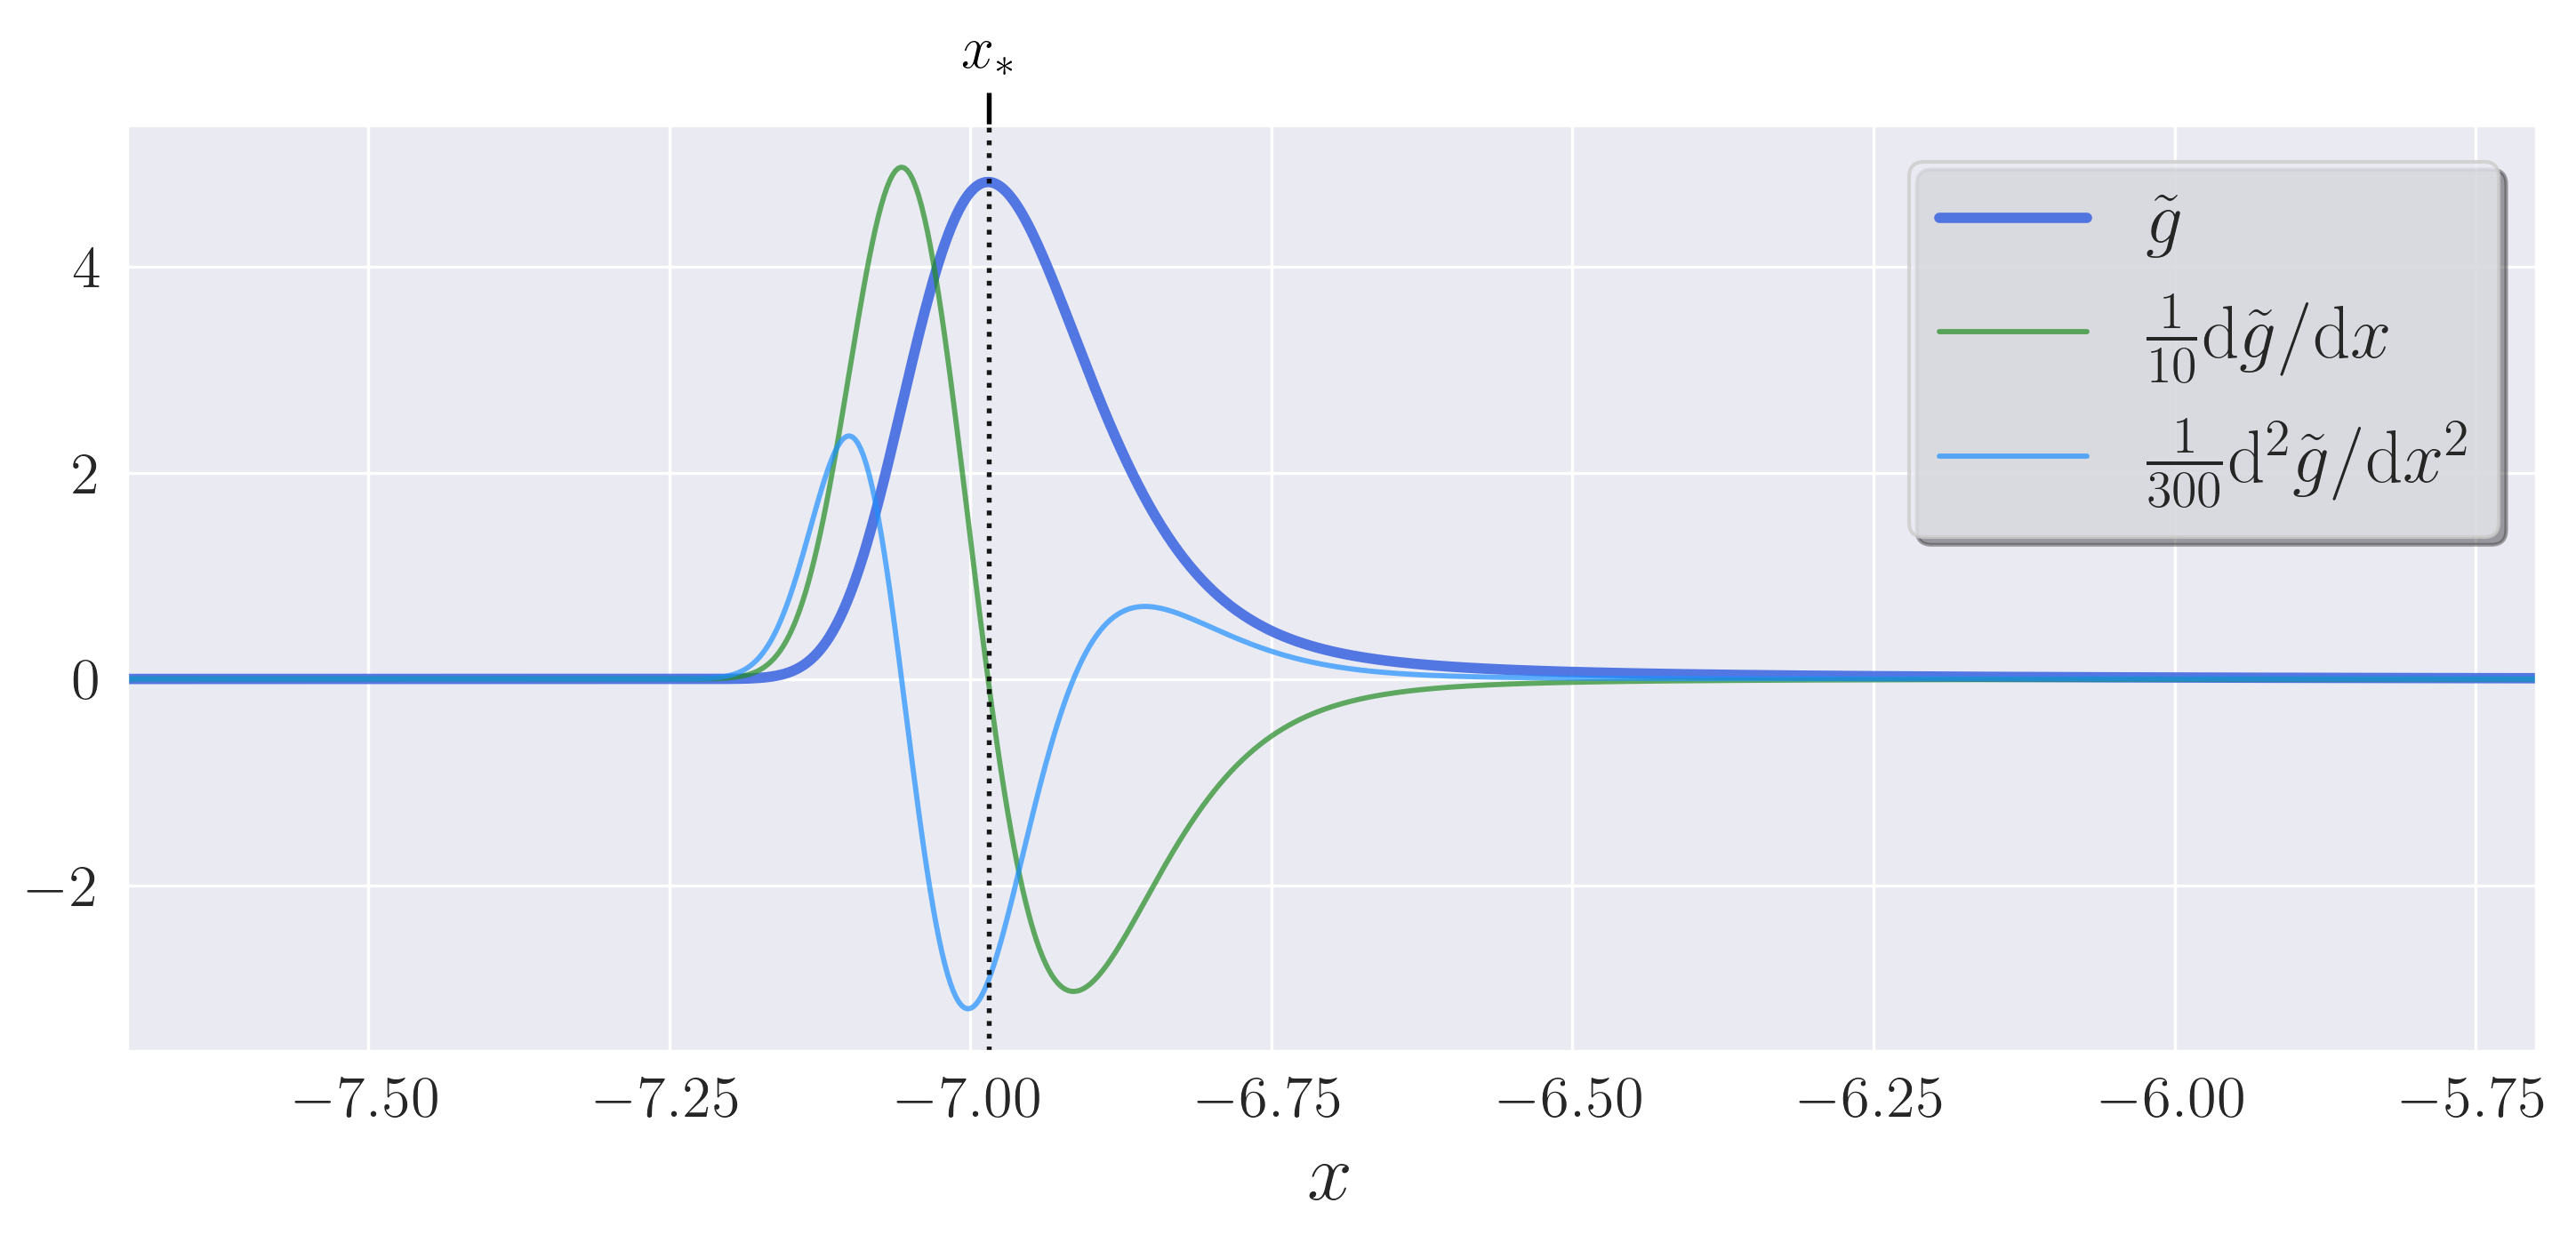
\includegraphics[width=\linewidth]{milestone2/visibility_function_misc.png} 
    \caption{\textcolor{blue}{The visibility function $\gt(x)$ and its derivatives $\dv{\gt(x)}{x}$ and $\dv[2]{\gt(x)}{x}$ as functions of logarithmic scale factor $x$.}} 
    \label[fig]{mil2:res:fig:visibility_function}
\end{figure}


\begin{table}[h]
    \setlength\tabcolsep{0pt} % let LaTeX figure out amount of inter-column whitespace
    % \begin{tabular*}{\linewidth}{@{\extracolsep{\fill}} l *{3}{d{2.4}} }
    \caption{The values of the logarithmic scale factor $x$, the redshift $z$ and the cosmic time $t$ corresponding to two events in the history of the universe.}
    \label[tab]{mil2:res:tab:time_of_events}
    \begin{tabular*}{\linewidth}{@{\extracolsep{\fill}} l *{3}{d{3.3}} l}
        \toprule
        % & \multicolumn{3}{c}{Time of event} \\
        & \multicolumn{1}{c}{$x$} & \multicolumn{1}{c}{$z$} & \multicolumn{1}{c}{$t$} & \\
        \midrule
        Last scattering surface & -555& 1000 & 51.06\text{~ka}& \\
        Recombination     & -555 & 1000 & 7.753\text{~Ga}& \\
        \midrule
        % Conformal time today: & \multicolumn{4}{c}{$\eta_0 = 46.32 c$~Ga}\\
        \multicolumn{2}{l}{FO free electron abundance today: }& \multicolumn{3}{c}{$X_{e0} = $}\\
        \multicolumn{2}{l}{Sound horison at decoupling: }& \multicolumn{3}{c}{$r_s(\eta_*) = $}\\
        \bottomrule
    \end{tabular*}
\end{table}